% Template for an EarthArXiv preprint of the manuscript.
% Includes the standard disclaimers and formatting that is required.
%
% This is the document structure. The actual content is written in:
% * abstract.tex: The abstract.
% * abstract-plain.tex: A plain language version of the abstract.
% * content.tex: The actual manuscript text (minus the abstract).
%
%%%%%%%%%%%%%%%%%%%%%%%%%%%%%%%%%%%%%%%%%%%%%%%%%%%%%%%%%%%%%%%%%%%%%%%%%%%%%%%
% Set a class and general configuration
\documentclass[onecolumn,10pt]{article}

%%%%%%%%%%%%%%%%%%%%%%%%%%%%%%%%%%%%%%%%%%%%%%%%%%%%%%%%%%%%%%%%%%%%%%%%%%%%%%%
% Set variables with the title, authors, etc.
\newcommand{\Title}{Supplementary files}
\newcommand{\TitleShort}{A short title}

\newcommand{\Year}{2023}
\newcommand{\SubmittedOn}{2023/02/28}
\newcommand{\PublishedOn}{2023/02/28}

\newcommand{\AuthorShort}{Uieda \textit{et al.}}
\newcommand{\Authors}{%
  Leonardo Uieda\textsuperscript{1},
  Santiago R. Soler\textsuperscript{2}
}
\newcommand{\Email}{contact-email@university.org}
\newcommand{\Corresponding}{%
  Corresponding author: Leonardo Uieda <\href{mailto:\Email}{\Email}>
}
\newcommand{\Affiliations}{%
  \textsuperscript{1} Universidade de São Paulo, Brazil;
  \textsuperscript{2} University of British Columbia, Canada;
}

\newcommand{\Journal}{Geochemistry, Geophysics, Geosystems}
\newcommand{\JournalDOI}{YYYYY/YYYYYYY}
\newcommand{\PreprintDOI}{XXXXX/XXXXXXX}
\newcommand{\ArchiveDOI}{DOI_FOR_THE_REPO_ARCHIVE}
\newcommand{\GitHubRepository}{compgeolab/paper-template}

\newcommand{\Keywords}{%
  keyword1; keyword2; keyword3;
}

%%%%%%%%%%%%%%%%%%%%%%%%%%%%%%%%%%%%%%%%%%%%%%%%%%%%%%%%%%%%%%%%%%%%%%%%%%%%%%%
% Import the required packages
\usepackage[utf8]{inputenc}
\usepackage[TU]{fontenc}
\usepackage[english]{babel}
\usepackage{amsmath}
\usepackage{amssymb}
\usepackage{graphicx}
\usepackage{hyperref}
\usepackage{fancyhdr}
\usepackage{orcidlink}
\usepackage{geometry}
\usepackage{booktabs}
\usepackage{microtype}
\usepackage{siunitx}
% To customize the title page
\usepackage{titling}
% For adding multiple authors
\usepackage{authblk}
% improved urls with proper hyphenation
\usepackage{xurl}
% Tweak the look of captions
\usepackage{caption}
% To control the style of section titles
\usepackage{titlesec}
% Import natbib and doi packages
\usepackage[round,authoryear,sort]{natbib}
% show dois as links on references
\usepackage{doi}
% Remove extra space between references
\usepackage{natbibspacing}
% Use a different font
\usepackage[scaled=1.1]{notomath}
% Icons and fonts (requires using xelatex or luatex)
\usepackage{fontawesome5}
\usepackage{academicons}
% Control the font size
\usepackage{anyfontsize}
\usepackage{setspace}
% To get the number of pages in the document
\usepackage{lastpage}
\usepackage{lipsum}
\usepackage{ragged2e}
\usepackage{mdframed}
% To define custom environments
\usepackage{environ}
% To control hyphenation for individual blocks of text
\usepackage{hyphenat}


%%%%%%%%%%%%%%%%%%%%%%%%%%%%%%%%%%%%%%%%%%%%%%%%%%%%%%%%%%%%%%%%%%%%%%%%%%%%%%%
% Configuration of the document

\geometry{%
  left=25mm,
  right=25mm,
  top=18mm,
  bottom=15mm,
  headsep=0mm,
  headheight=0mm,
  footskip=7mm,
  includehead=true,
  includefoot=true
}

% Control line and table row spacing
\onehalfspacing
\renewcommand{\arraystretch}{1.5}

% Set the spacing between bibliography entries (requires natbib)
\setlength{\bibsep}{0pt}

% Custom colors
\definecolor{darkgray}{gray}{0.4}
\definecolor{mediumgray}{gray}{0.5}
\definecolor{lightgray}{gray}{0.9}
\definecolor{mediumblue}{HTML}{2060c2}
\definecolor{lightblue}{HTML}{f7faff}

% Configure captions
\captionsetup[table]{position=below,skip=0pt}
\captionsetup{labelfont=bf,font={small,color=darkgray},skip=10pt}

% Make urls use the same font as every other text
\urlstyle{same}

% Configure hyperref and add PDF metadata
\hypersetup{
    colorlinks,
    allcolors=mediumblue,
    pdftitle={\Title},
    pdfauthor={\AuthorShort},
    breaklinks=true,
}

% Configure header and footer
% Inspired by LaPreprint: https://github.com/roaldarbol/LaPreprint
\newcommand{\Separator}{\hspace{3pt}|\hspace{3pt}}
\newcommand{\FooterFont}{\footnotesize\color{mediumgray}}
\pagestyle{fancy}
\fancyhf{}
\lfoot{%
  \FooterFont{}
  \AuthorShort{} (\Year)
  \Separator{}
  \TitleShort
}
\rfoot{%
  \FooterFont{}
  EarthArXiv
  \Separator{}
  \thepage\space of\space \pageref*{LastPage}
}
\renewcommand{\headrulewidth}{0pt}
\renewcommand{\footrulewidth}{1pt}
\preto{\footrule}{\color{lightgray}}
\fancypagestyle{plain}{%
  \fancyhf{}
  \lfoot{%
    \FooterFont{}
    \faCreativeCommons\faCreativeCommonsBy
    \Separator{}
    \textcopyright{} \Year{} The Authors
  }
  \rfoot{%
    \FooterFont{}
    doi:\href{https://doi.org/\PreprintDOI}{\PreprintDOI}
    \Separator{}
    EarthArXiv
    \Separator{}
    \thepage\space of\space \pageref*{LastPage}
  }
}

% Define fancy text boxes
\NewEnviron{summarybox}{%
  \mdfdefinestyle{summarybox_}{%
    leftline=true,
    rightline=false,
    topline=false,
    bottomline=false,
    linewidth=2pt,
    linecolor=mediumblue,
    backgroundcolor=lightblue,
    innertopmargin=12pt,
    innerbottommargin=12pt,
    innerleftmargin=12pt,
    innerrightmargin=12pt,
    skipbelow=5pt,
    skipabove=5pt,
  }
  \newmdenv[style=summarybox_]{summarybox_}
  \begin{summarybox_}
    \footnotesize
    \BODY
  \end{summarybox_}
}

%%%%%%%%%%%%%%%%%%%%%%%%%%%%%%%%%%%%%%%%%%%%%%%%%%%%%%%%%%%%%%%%%%%%%%%%%%%%%%%
\begin{document}

\thispagestyle{plain}
\begin{FlushLeft}
  \begin{spacing}{2}
    {\LARGE\bfseries \Title}
  \end{spacing}
  {\color{lightgray}\hrule height 1.5pt}
  \vspace{0.3cm}
  \Authors
  \\[0.2cm]
  {\footnotesize \Affiliations}
  \newline
  {\footnotesize \Corresponding}
  \\[0.2cm]
  {\footnotesize
    Received in original form on \SubmittedOn.
    %Published in final form on \PublishedOn.
  }
\end{FlushLeft}

\begin{summarybox}
  \noindent
  \textbf{Disclaimer:}
  %This is a non-peer reviewed preprint of an article submitted for publication
  %in \textit{\Journal{}}. It is available from EarthArXiv at
  %\url{https://doi.org/\PreprintDOI}.
  %%%%%%%%%%%%%%%%%%%%%%%%%%%%%%%%%%%%%%%%%%%%%%%%%%%%%%%%%%%%%%%%%%%%%%%%%%%%%
  % Comment the above and uncomment below after publication in a journal
  %%%%%%%%%%%%%%%%%%%%%%%%%%%%%%%%%%%%%%%%%%%%%%%%%%%%%%%%%%%%%%%%%%%%%%%%%%%%%
  This is a peer-reviewed author-produced postprint of the article
  ``\AuthorShort{} (\Year). \Title. \textit{\Journal}.
  doi:\href{https://doi.org/\JournalDOI}{\JournalDOI}''.
  The postprint is available from EarthArXiv at
  \url{https://doi.org/\PreprintDOI}.
  %%%%%%%%%%%%%%%%%%%%%%%%%%%%%%%%%%%%%%%%%%%%%%%%%%%%%%%%%%%%%%%%%%%%%%%%%%%%%
  \\[0.25cm]
  \noindent
  \textbf{Open research:}
  The source code used to generate all of the results presented in this
  research can be freely accessed and reused under the terms of an open license.
  You can find it at \url{https://doi.org/\ArchiveDOI} and
  \url{https://github.com/\GitHubRepository}.
  \\[0.25cm]
  \noindent
  \textbf{Keywords:} \Keywords{}
  \\[0.25cm]
  \noindent
  \textbf{\textcopyright{} \Year{} The Authors.}
  Available under the \href{https://creativecommons.org/licenses/by/4.0/}{Creative Commons Attribution 4.0 International License}
  \faCreativeCommons\faCreativeCommonsBy{}.
\end{summarybox}

\section*{\normalsize Plain language summary}
\begingroup
  \setstretch{1.1} \small \lipsum[3]
 \par
\endgroup

\section*{\normalsize Abstract}
\begingroup
  \setstretch{1.1} \small Magnetic microscopy mapping for paleomagnetic studies has attracted considerable attention in recent years due to its high accuracy and robustness. However, due to the nature of the magnetic field, it is difficult to accurately estimate the magnetic source's position and dipole moment. This study proposes a new methodology to mitigate the magnetic sources' interference and enhance the precision of the inversion analyses proposed. The proposed methodology is based on refining the isolation of the primary signal and integrating the "interfering sources" algorithm, which addresses one of the previous code's limitations. Moreover, the proposed methodology was applied to synthetic data to assess the algorithm's reliability and precision, reinforcing the advancement of paleomatrix data analysis and setting a definitive path for future enhancements. \par
\endgroup


%%%%%%%%%%%%%%%%%%%%%%%%%%%%%%%%%%%%%%%%%%%%%%%%%%%%%%%%%%%%
\subsubsection{Vertical component magnetic field ($\mathbf{b_z}$)}\label{section_bz}
After identifying the position of the source, assuming it is a dipole, we can utilize the modified approach from \citet{Oliveira2015Estimation} to calculate the dipole moment vector, denoted as 
\textbf{m}. The magnetic induction vector $\mathbf{b_z}$ for a dipole is given by

\begin{equation}
\label{eq_dipole_bz}
\mathbf{b_z}
= \dfrac{\mu_0}{4\pi}
\begin{bmatrix}
\dfrac{\partial^2}{\partial z \partial x} \dfrac{1}{r}
& \dfrac{\partial^2}{\partial z \partial y} \dfrac{1}{r}
& \dfrac{\partial^2}{\partial z \partial z} \dfrac{1}{r}
\end{bmatrix}
\begin{bmatrix}
m_x \\ m_y \\ m_z
\end{bmatrix}
= \dfrac{\mu_0}{4\pi} \mathbf{M_z}\,\mathbf{m}
\ .
\end{equation}

To address the mutual interference of magnetic sources, a method involves simultaneously solving the magnetic moment inversion for all "L" identified, therefore the Equation \ref{eq_dipole_bz} becomes


\begin{equation}
% \footnotesize
\label{eq_dipole_bz_all}
\dfrac{\mu_0}{4\pi}
{\begin{bmatrix}
\dfrac{\partial^2}{\partial z \partial x} \dfrac{1}{r_{1,1}}
& \dfrac{\partial^2}{\partial z \partial y} \dfrac{1}{r_{1,1}}
& \dfrac{\partial^2}{\partial z \partial z} \dfrac{1}{r_{1,1}}
& \hdots
& \dfrac{\partial^2}{\partial z \partial x} \dfrac{1}{r_{1,L}}
& \dfrac{\partial^2}{\partial z \partial y} \dfrac{1}{r_{1,L}}
& \dfrac{\partial^2}{\partial z \partial z} \dfrac{1}{r_{1,L}} \\
\\

& 
& 
& \vdots
& 
& 
&  \\
\\
\dfrac{\partial^2}{\partial z \partial x} \dfrac{1}{r_{N,1}}
& \dfrac{\partial^2}{\partial z \partial y} \dfrac{1}{r_{N,1}}
& \dfrac{\partial^2}{\partial z \partial z} \dfrac{1}{r_{N,1}}
& \hdots
& \dfrac{\partial^2}{\partial z \partial x} \dfrac{1}{r_{N,L}}
& \dfrac{\partial^2}{\partial z \partial y} \dfrac{1}{r_{N,L}}
& \dfrac{\partial^2}{\partial z \partial z} \dfrac{1}{r_{N,L}} \\
\end{bmatrix}}_{N \times 3L}
{\begin{bmatrix}
{m_x}_1 \\ {m_y}_1 \\ {m_z}_1 \\ \vdots \\{m_x}_L \\ {m_y}_L \\ {m_z}_L \\
\end{bmatrix}}_{3L \times 1}
=
{\begin{bmatrix}
{b_z}_1 \\ {b_z}_2 \\ {b_z}_3 \\ \vdots \\{b_z}_N 
\end{bmatrix}}_{N \times 1}.
\end{equation} \bigskip

In which $r_{i,j} = \sqrt{(x_i - {x_c}_j)^2 + (y_i - {y_c}_j)^2 + (z_i - {z_c}_j)^2}$ is the Cartesian distance between the i-th, $i=1, 2, \hdots N$, observation point $b_z (x_i, y_i, z_i)$ and the j-th, $j=1, 2, \hdots L$, point source $({x_c}_j, {y_c}_j, {z_c}_j)$ and $\mu_0$ is the vacuum magnetic permeability. While the three second-order derivatives in Equation~\ref{eq_dipole_bz_all} are:

\begin{equation}
% \footnotesize
\begin{aligned}
\dfrac{\partial^2}{\partial z \partial x} \dfrac{1}{r_{i,j}} &=
\dfrac{3(z_i - {z_c}_j)(x_i - {x_c}_j)}{{r_{i,j}}^5}\ ,
\\
\dfrac{\partial^2}{\partial z \partial y} \dfrac{1}{r_{i,j}} &=
\dfrac{3(z_i - {z_c}_j)(y_i - {y_c}_j)}{{r_{i,j}}^5}\ ,
\\
\dfrac{\partial^2}{\partial z \partial z} \dfrac{1}{r_{i,j}} &=
\dfrac{3(z_i - {z_c}_j)^2}{{r_{i,j}}^5} - \dfrac{1}{{r_{i,j}}^3}\ .
\end{aligned}
\end{equation}   \bigskip

The Equation \ref{eq_dipole_bz_all} can be expressed in matrix form as

\begin{equation}
\label{qdhqM4s9Ln}
\mathbf{M_z} \mathbf{m} = \mathbf{b_z}^{pred} \ .
\end{equation}

The dipole moment vector that best fits
a set of $N$ observations of the vertical component of the magnetic field
$\mathbf{b_z}^{obs}$ is given by minimizing the misfit function using a least-squares estimator

\begin{equation}
\label{uV9pRVYO4l}
\Phi (\mathbf{m}) = \| \mathbf{b_z}^{obs} - \mathbf{b_z}^{pred} \|^2 = (\mathbf{b_z}^{obs} - \mathbf{M_z}\mathbf{m})^T  (\mathbf{b_z}^{obs} - \mathbf{M_z}\mathbf{m})\ .
\end{equation}

The dipole moment vector that minimizes $\Phi (\mathbf{m})$ can be found by solving the linear equation system

\begin{equation}
 \mathbf{m} = {\left ( \mathbf{M_z}^T \mathbf{M_z} \right )}^{-1} \mathbf{M_z}^T\mathbf{b_z}^{obs}\ .
\end{equation}

Therefore, taking into account all their mutual signal interference in the N observed data increases further the trade-off between accuracy and run time.



\subsubsection{Vertical derivative of $\mathbf{b_z}$}

%An alternative method to enhance the inversion process involves utilizing the first derivative of \( b_z \). 

Applying derivatives in geophysical investigations offers improved sensitivity to shallow sources, enabling the isolation and detailed analysis of local geological features. The flexibility and versatility inherent in fractional order derivatives allow for precise adjustments in the separation process, enabling accurate estimation of the local field, such as shown by \citet{Florio2022}. In the latter, the vertical derivative serves as a straightforward and stable tool for regional-residual separation, even in regions with restricted spatial extent. This contributes to the precise prediction and isolation of local field characteristics. 

We obtained the partial derivative ($\partial_z f$) of the magnetic field ($f$) concerning $z$ using a second-order accurate central finite-difference scheme based on two upward continuation applications

\begin{equation}
\partial_z f(x, y, z) \approx
\dfrac{f(x + \Delta z, y, z) - f(x - \Delta z, y, z)}{2 \Delta z}
\ .
\end{equation}

This derivative functions as a high-pass filter, effectively reducing the potential interference caused by the long-wavelength signal of the stronger source with weaker sources. We can obtain \( \frac{b_z}{\partial z} \) by differentiating both sides of Equation~\ref{eq_dipole_bz_all} with respect to \( z \):



\begin{equation}
\footnotesize
\label{eq_dipole_bz_z_deriv}
\dfrac{\mu_0}{4\pi}
% \scriptsize
{\begin{bmatrix}
\dfrac{\partial^2}{\partial z \partial x \partial z} \dfrac{1}{r_{1,1}}
& \dfrac{\partial^2}{\partial z \partial y \partial z} \dfrac{1}{r_{1,1}}
& \dfrac{\partial^2}{\partial z \partial z \partial z} \dfrac{1}{r_{1,1}}
& \hdots
& \dfrac{\partial^2}{\partial z \partial x \partial z} \dfrac{1}{r_{1,L}}
& \dfrac{\partial^2}{\partial z \partial y \partial z} \dfrac{1}{r_{1,L}}
& \dfrac{\partial^2}{\partial z \partial z \partial z} \dfrac{1}{r_{1,L}} \\
\\

& 
& 
& \vdots
& 
& 
&  \\
\\
\dfrac{\partial^2}{\partial z \partial x \partial z} \dfrac{1}{r_{N,1}}
& \dfrac{\partial^2}{\partial z \partial y \partial z} \dfrac{1}{r_{N,1}}
& \dfrac{\partial^2}{\partial z \partial z \partial z} \dfrac{1}{r_{N,1}}
& \hdots
& \dfrac{\partial^2}{\partial z \partial x \partial z} \dfrac{1}{r_{N,L}}
& \dfrac{\partial^2}{\partial z \partial y \partial z} \dfrac{1}{r_{N,L}}
& \dfrac{\partial^2}{\partial z \partial z \partial z} \dfrac{1}{r_{N,L}} \\
\end{bmatrix}}_{N \times 3L}
{\begin{bmatrix}
{m_x}_1 \\ {m_y}_1 \\ {m_z}_1 \\ \vdots \\{m_x}_L \\ {m_y}_L \\ {m_z}_L \\
\end{bmatrix}}_{3L \times 1}
=
{\begin{bmatrix}
\frac{{b_z}_1}{ \partial z} \\ \frac{{b_z}_2}{ \partial z} \\ \frac{{b_z}_3}{ \partial z} \\ \vdots \\\frac{{b_z}_N}{ \partial z}
\end{bmatrix}}_{N \times 1}.
\end{equation} \bigskip

In Equation~\ref{eq_dipole_bz_z_deriv}, the three third-order derivatives are given by:

\begin{equation}
% \footnotesize
\begin{aligned}
\dfrac{\partial^2}{\partial z \partial x \partial z} \dfrac{1}{r_{i,j}} &=
\dfrac{3(x_i - {x_c}_j)}{{r_{i,j}}^5} - \dfrac{15(x_i - {x_c}_j)(z_i - {z_c}_j)^2}{{r_{i,j}}^7}\ ,
\\
\dfrac{\partial^2}{\partial z \partial y \partial z} \dfrac{1}{r_{i,j}} &=
\dfrac{3(y_i - {y_c}_j)}{{r_{i,j}}^5} - \dfrac{15(y_i - {y_c}_j)(z_i - {z_c}_j)^2}{{r_{i,j}}^7}\ ,
\\
\dfrac{\partial^2}{\partial z \partial z \partial z} \dfrac{1}{r_{i,j}} &=
\dfrac{9(z_i - {z_c}_j)}{{r_{i,j}}^5} - \dfrac{15(z_i - {z_c}_j)^3}{{r_{i,j}}^7}\ .
\end{aligned}
\end{equation}   \bigskip

As demonstrated in Section \ref{section_bz}, Equation \ref{eq_dipole_bz_z_deriv} can also be expressed in matrix linear form

\begin{equation}
\label{qdhqM4s9Ln1}
\mathbf{{M_{zz}}} \mathbf{m} = \mathbf{{b_{zz}}}^{pred} \ .
\end{equation}

And the dipole moment vector $(\mathbf{m})$ is determined by solving

\begin{equation}
 \mathbf{m} = {\left ( \mathbf{{M_{zz}}}^T \mathbf{{M_{zz}}} \right )}^{-1} \mathbf{{M_{zz}}}^T\mathbf{{b_{zz}}}^{obs}\ .
 %\mathbf{m} = {\left ( \mathbf{{M_z}_{_z}}^T \mathbf{{M_z}_{_z}} \right )}^{-1} \mathbf{{M_z}_{_z}}^T\mathbf{{b_z}_{_z}}^{obs}\ .
\end{equation}


\subsection{Subset optimization for inversion}

Magnetic inversion is a crucial technique used in magnetic microscopy to gain insights into the internal structures and magnetic features of microscopic materials. However, dealing with extensive datasets (Figure \ref{methodology}a) has become a computational challenge, especially with the progressive refinement in spatial resolution of magnetic microscopes. Thus, strategic approaches are required to enhance efficiency. In this section, we will outline a key aspect of our methodology, which is the optimization of magnetic inversion through the careful selection of a subset of data.

It is possible to reduce the time necessary to perform magnetic inversion by eliminating irrelevant data points that do not contribute significantly to the analysis. This involves identifying and extracting specific regions within the dataset where magnetic sources of interest are expected while minimizing the influence of noisy or irrelevant areas (Figure \ref{methodology}b). By focusing on these targeted regions, we can expedite the inversion process and also improve the accuracy and reliability of the results. It is important to note that selecting a subset of data is a mandatory part of the iterative Euler deconvolution process. The methodology for interfering sources inversion seamlessly integrates this step, making it more efficient and cohesive.


\begin{figure}[tb!]
  \centering
  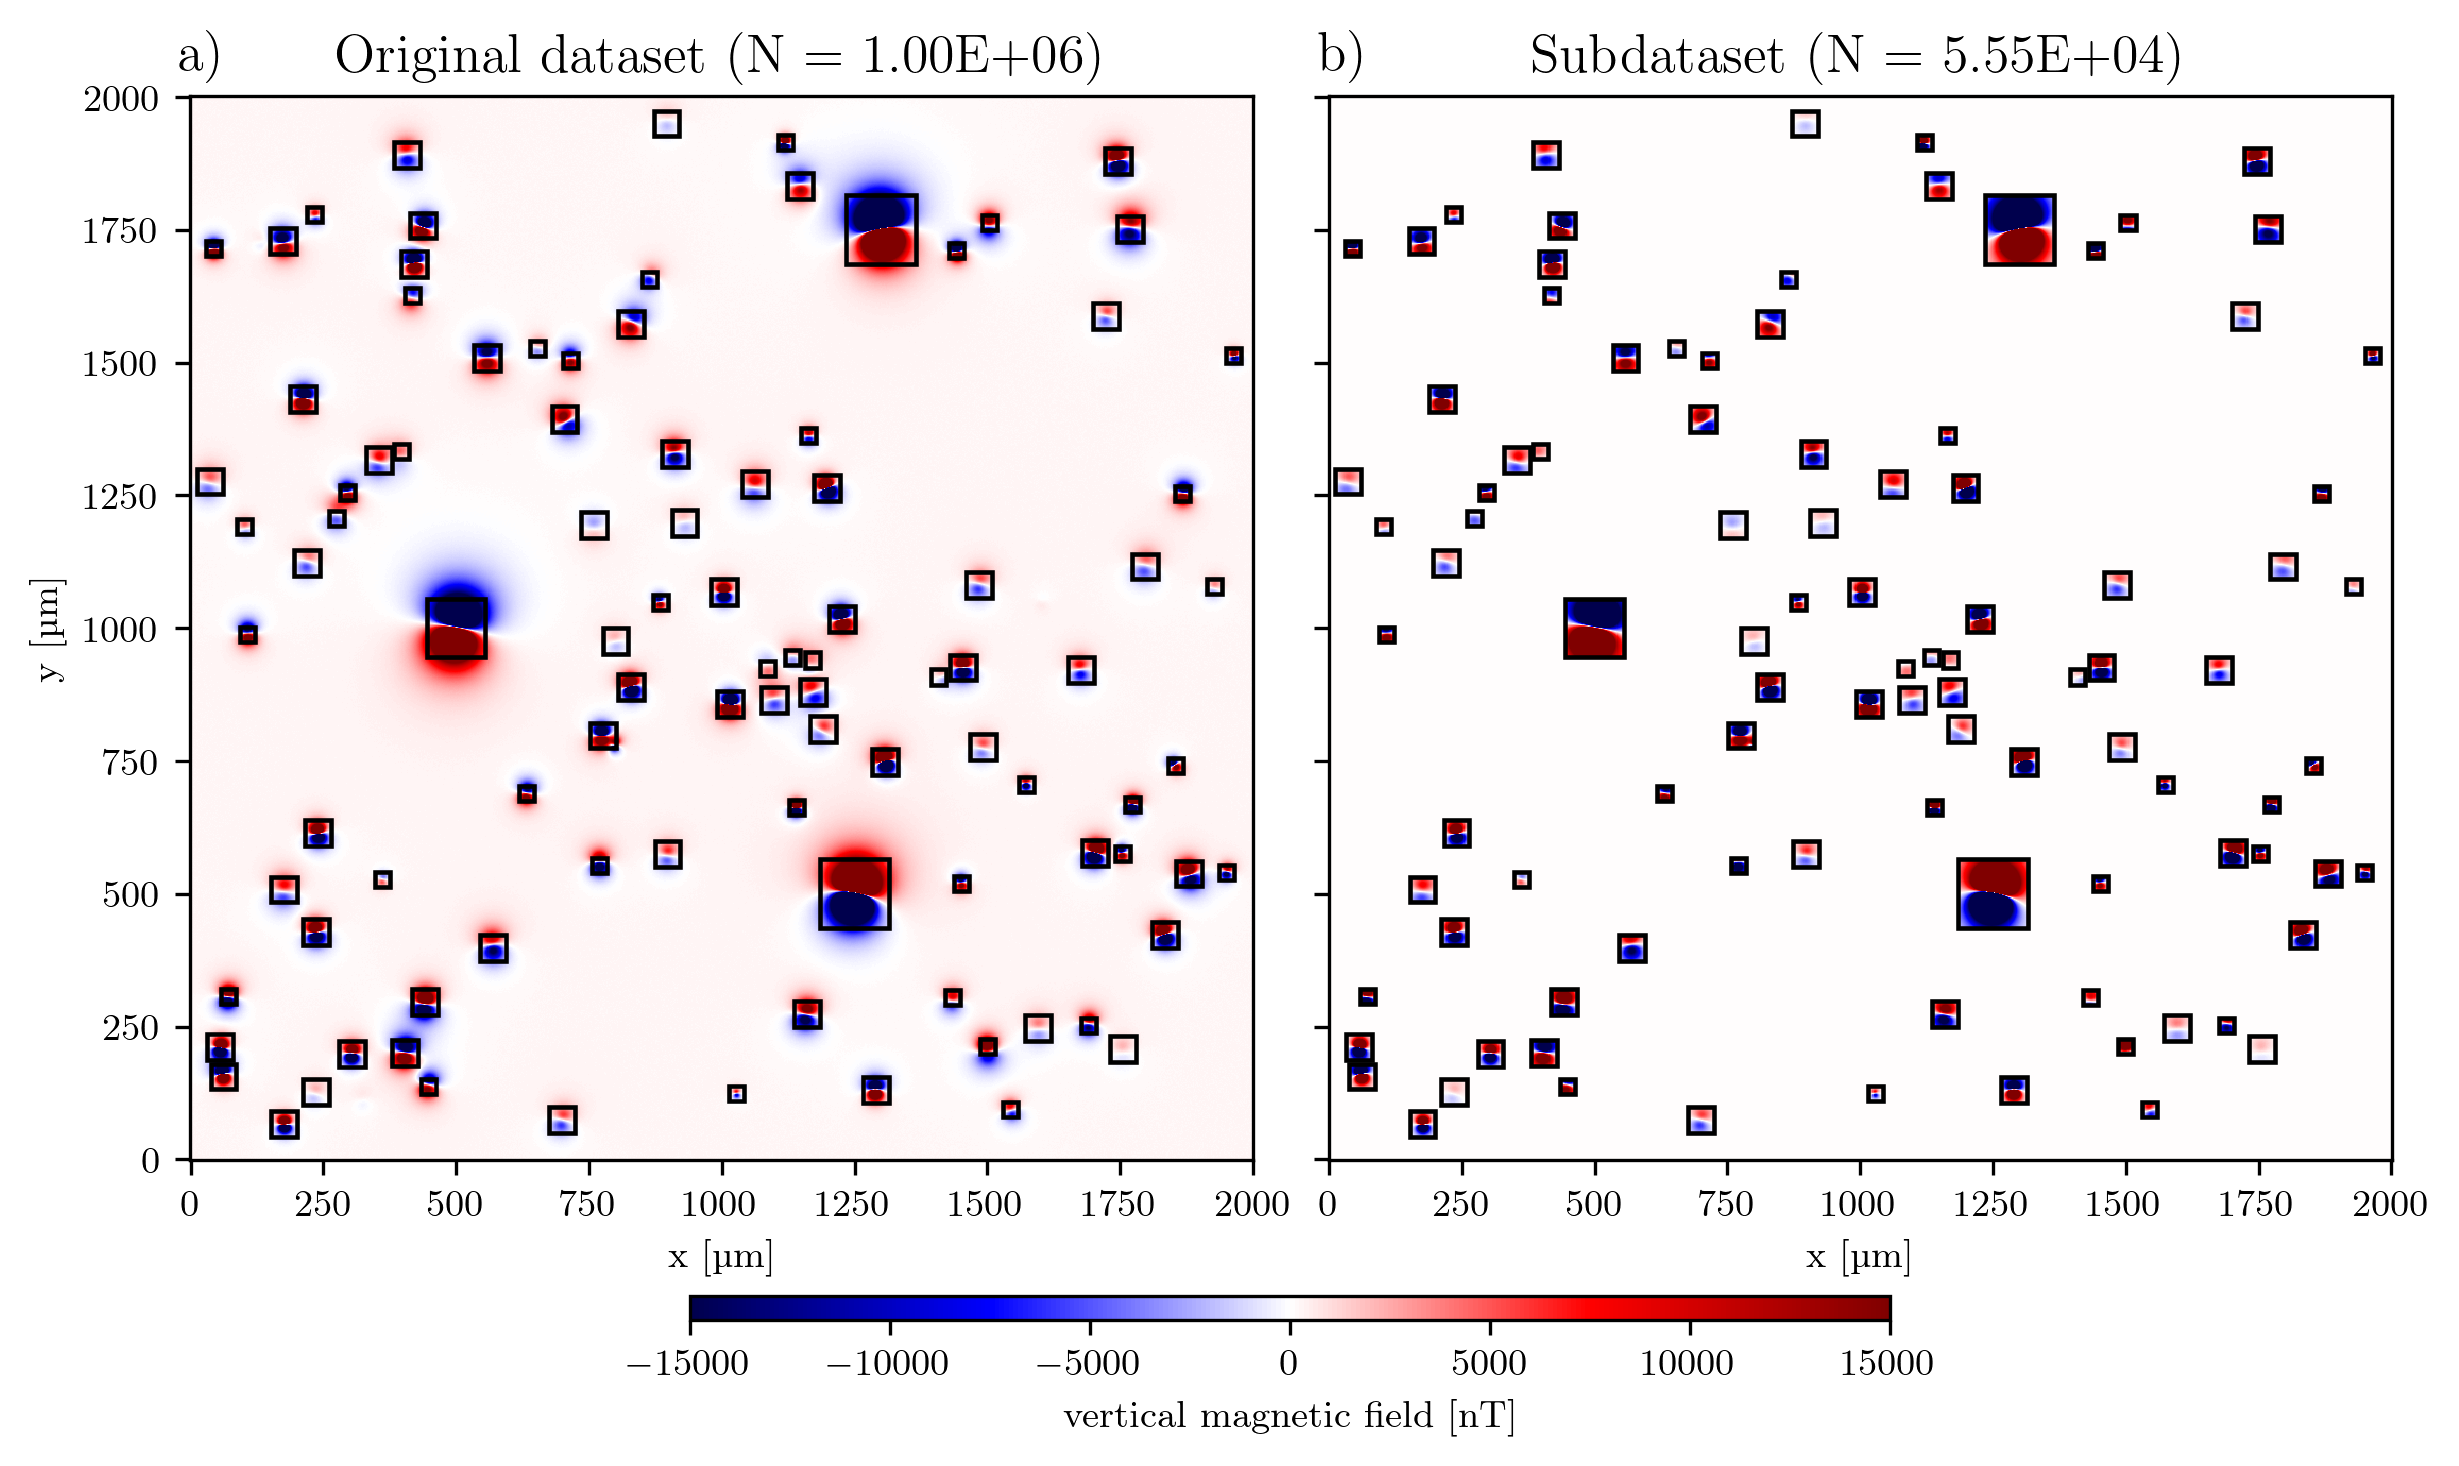
\includegraphics[width=1\linewidth]{figures/methodology.png}
  \caption{
    Tackling computational challenges in magnetic microscopy with extensive datasets.
    a) Complete synthetic dataset featuring all N observation points including areas lacking relevant information.
    b) Streamlining data through pre-selected windows reduces the dataset size for inversion, ensuring efficiency without compromising final results.
      }
  \label{methodology}
\end{figure}

%%%%%%%%%%%%%%%%%%%%%%%%%%%%%%%%%%%%%%%%%%%%%%%%%%%%%%%%%%%%%%%%%%%%%%%%%%%%%%%



\section{Synthetic data application}

As mentioned, this study aims to deal with the mutual interference between the magnetic sources. The proposed methodologies were applied to two sets of complex synthetic data to assess the algorithm's performance, the datasets were designed to evaluate the methodology under different conditions. The inversion workflow was tested for its efficiency in the presence of interfering sources for further comparison with the methodology proposed by  \citet{Souza-Junior2023b}.

\begin{enumerate}
\item \textbf{Method validation with interfering sources:}
The first model scenario features several dipole sources with different moment magnitude, inclination, and declination clustered around two stable directions. The vertical magnetic field ($b_z$) generated from these sources is corrupted by both low and high-frequency noise, simulating real-world magnetic microscopy data. 

\item \textbf{Shifted magnetic field acquisition:}
The second model replicates the conditions of the first scenario, maintaining the same simulation parameters for the sources. However, in this case, the magnetic field data undergoes a positive shift to simulate the acquisition process in magnetic microscopy with a shifted baseline. This scenario provides insights into the algorithm's robustness and accuracy when faced with a systematically shifted magnetic field, as encountered in certain microscopic magnetic data acquisition setups.
\end{enumerate}

\subsection{Method validation with interfering sources}\label{non-shifted}

We analyze how the method works by simulating a complex scenario containing 103 magnetic sources randomly distributed across the imaged area of a synthetic thin section measuring $\qty{2000}{\um} \times \qty{2000}{\um}$. The synthetic $b_z$ data were generated on a regular grid with a spacing of $\qty{2}{\um}$ and a $\qty{5}{\um}$ sensor-sample distance. To make the simulation more realistic, we intentionally incorporated a high-frequency pseudo-random noise, with a zero mean and a standard deviation of $\qty{50}{\nano\tesla}$, and low-frequency noise. In real ferromagnetic particles, the Natural Remanent Magnetization (NRM) exhibits individual variations but tends to align with the inducing field direction. To capture this variability in our synthetic data, we sampled the dipole moment directions from two pseudo-random Gaussian distributions. The first group of sources ($M = 70$) was sampled from a distribution with a mean of $D = \ang{0}\pm\ang{10}$ and $I = \ang{0}\pm\ang{10}$. The second group of sources ($M = 30$) was sampled from a distribution with a mean of $D = \ang{180}\pm\ang{10}$ and $I = \ang{0}\pm\ang{10}$. These sources have distinct depths (between 1 and $\qty{20}{\um}$) and magnetic moment intensities (from $10^{-14}$ to $\qty{e-12}{\ampere\m\squared}$). Additionally, to further emulate the complexities observed in real data measurements, we manually introduced three deep-seated sources with higher dipole moments ($5 \times 10^{-11}$). 

The inversion for this synthetic data was solved using both the standard method \citep{Souza-Junior2023b} and the proposed interfering sources methodologies. A summary of the comparison between the classic Euler method and the iterative approach revealed noteworthy results in the context of the analysis of the provided synthetic data. Upon applying the iterative Euler deconvolution method, a significant enhancement in the precision of the magnetic source position is observed when compared to the Euler deconvolution in the standard method. Figure~\ref{euler1}a illustrates the detected sources, showcasing the algorithm's effectiveness in identifying regions of interest. Figures ~\ref{euler1}b and ~\ref{euler1}c show the results obtained by the standard and iterative Euler methods, respectively. It becomes evident that the iterative method yields more accurate and refined estimates. This increase in accuracy is crucial, especially in scenarios where stronger magnetic sources can distort the magnetic field anomaly of weaker sources. Although this new methodology can markedly increase the accuracy in the estimated position for virtually all sources, the biggest errors are still related to clustered sources.
%However, it is important to note that the enhanced precision with the iterative method comes at the cost of increased computational time, presenting a trade-off between superior results and computational efficiency.

\begin{figure}[tb!]
  \centering
  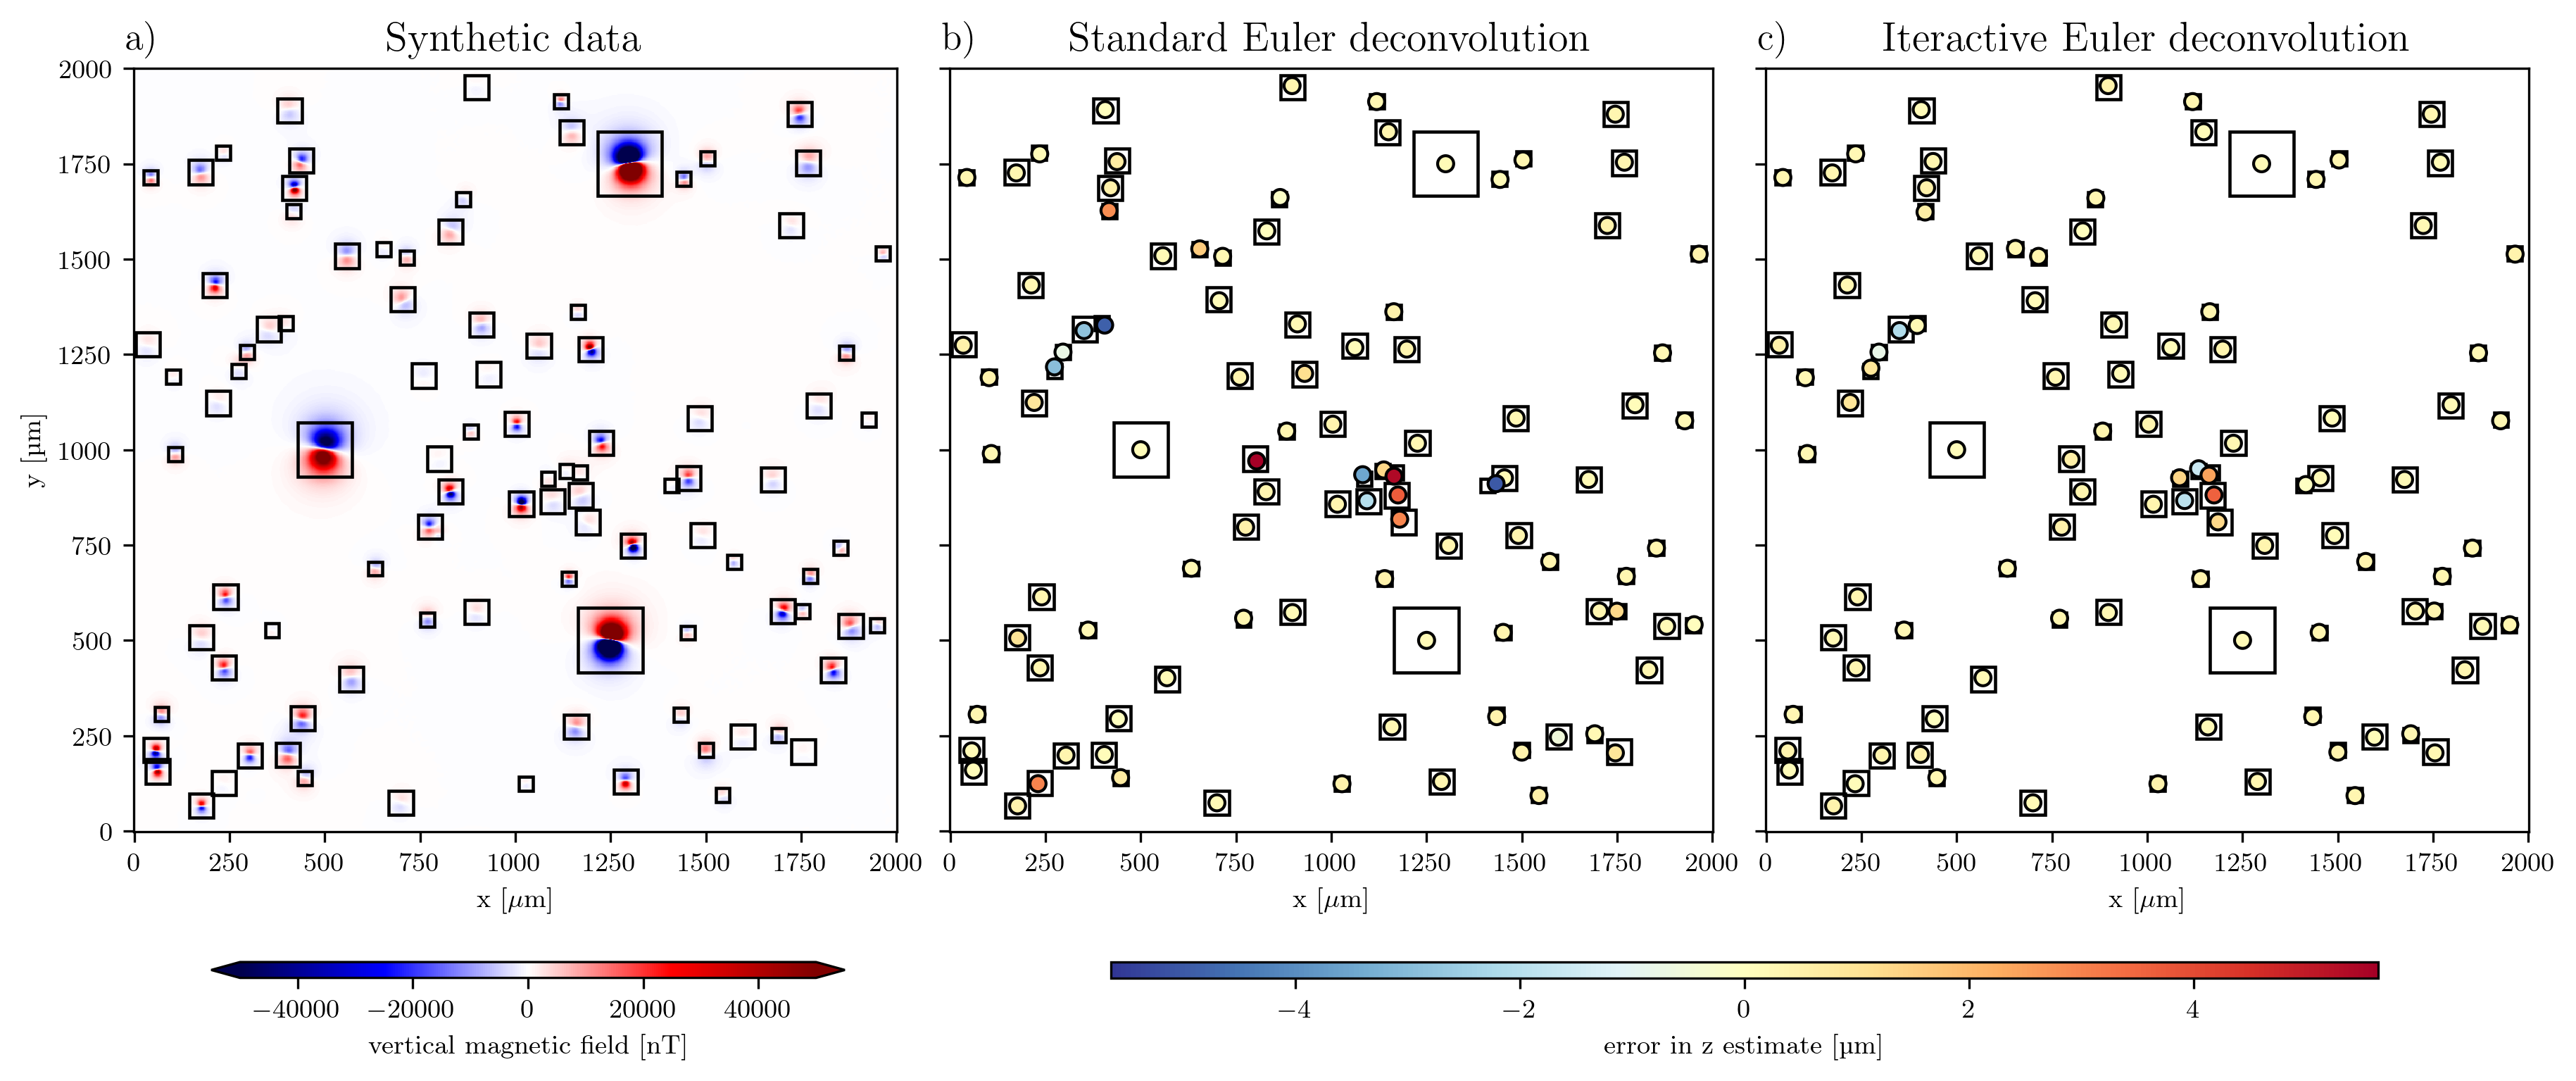
\includegraphics[width=1\linewidth]{figures/euler-comparion-1.png}
  \caption{
    % Addressing computational challenges in magnetic microscopy with extensive datasets.
    % a) Complete synthetic dataset featuring all N observation points including areas lacking relevant information.
    % b) Streamlining data through pre-selected windows reduces the dataset size for inversion, ensuring efficiency without compromising final results.
      }
  \label{euler1}
\end{figure}

These iterative Euler estimated positions were used for the magnetic inversion due to their better results except for the standard method results, which were kept unchanged from the results presented by \citet{Souza-Junior2023b}. Figure~\ref{inversion1} summarizes the comparison concerning the angular misfit, the magnetic moment misfit, and the r-squared score, respectively, for the standard (Figures~\ref{inversion1}a-c), iterative (Figures~\ref{inversion1}d-f) interfering sources using $b_z$ (Figures~\ref{inversion1}g-i), and interfering sources using the vertical derivative (Figures~\ref{inversion1}j-l). Overall, as predicted, every single interfering source method outperformed the standard one in all three of the measured parameters. It is worth mentioning that the iterative (Figures~\ref{inversion1}d) and the $b_{zz}$ interfering sources (Figures~\ref{inversion1}j) yield the best results for the angular misfit, with barely any difference, and also for the r-squared score. Nevertheless, the $b_{z}$ interfering sources technique shows slightly better results for the magnetic moment misfit. Although displaying better results than the standard method, none of the proposed methodologies are capable of dealing with tightly clustered sources, especially for the magnetic moment misfit. This observation might have its cause inherited rooted in the limitations of the Euler deconvolution, even after all the improvement of the iterative Euler deconvolution (Figures~\ref{euler1}c), which triggers the ambiguity between the source's depth with its magnetic intensity. This example shows that all proposed methodologies can be applied to magnetic microscopy yielding better results than the standard method.



\begin{figure}[tb!]
  \centering
  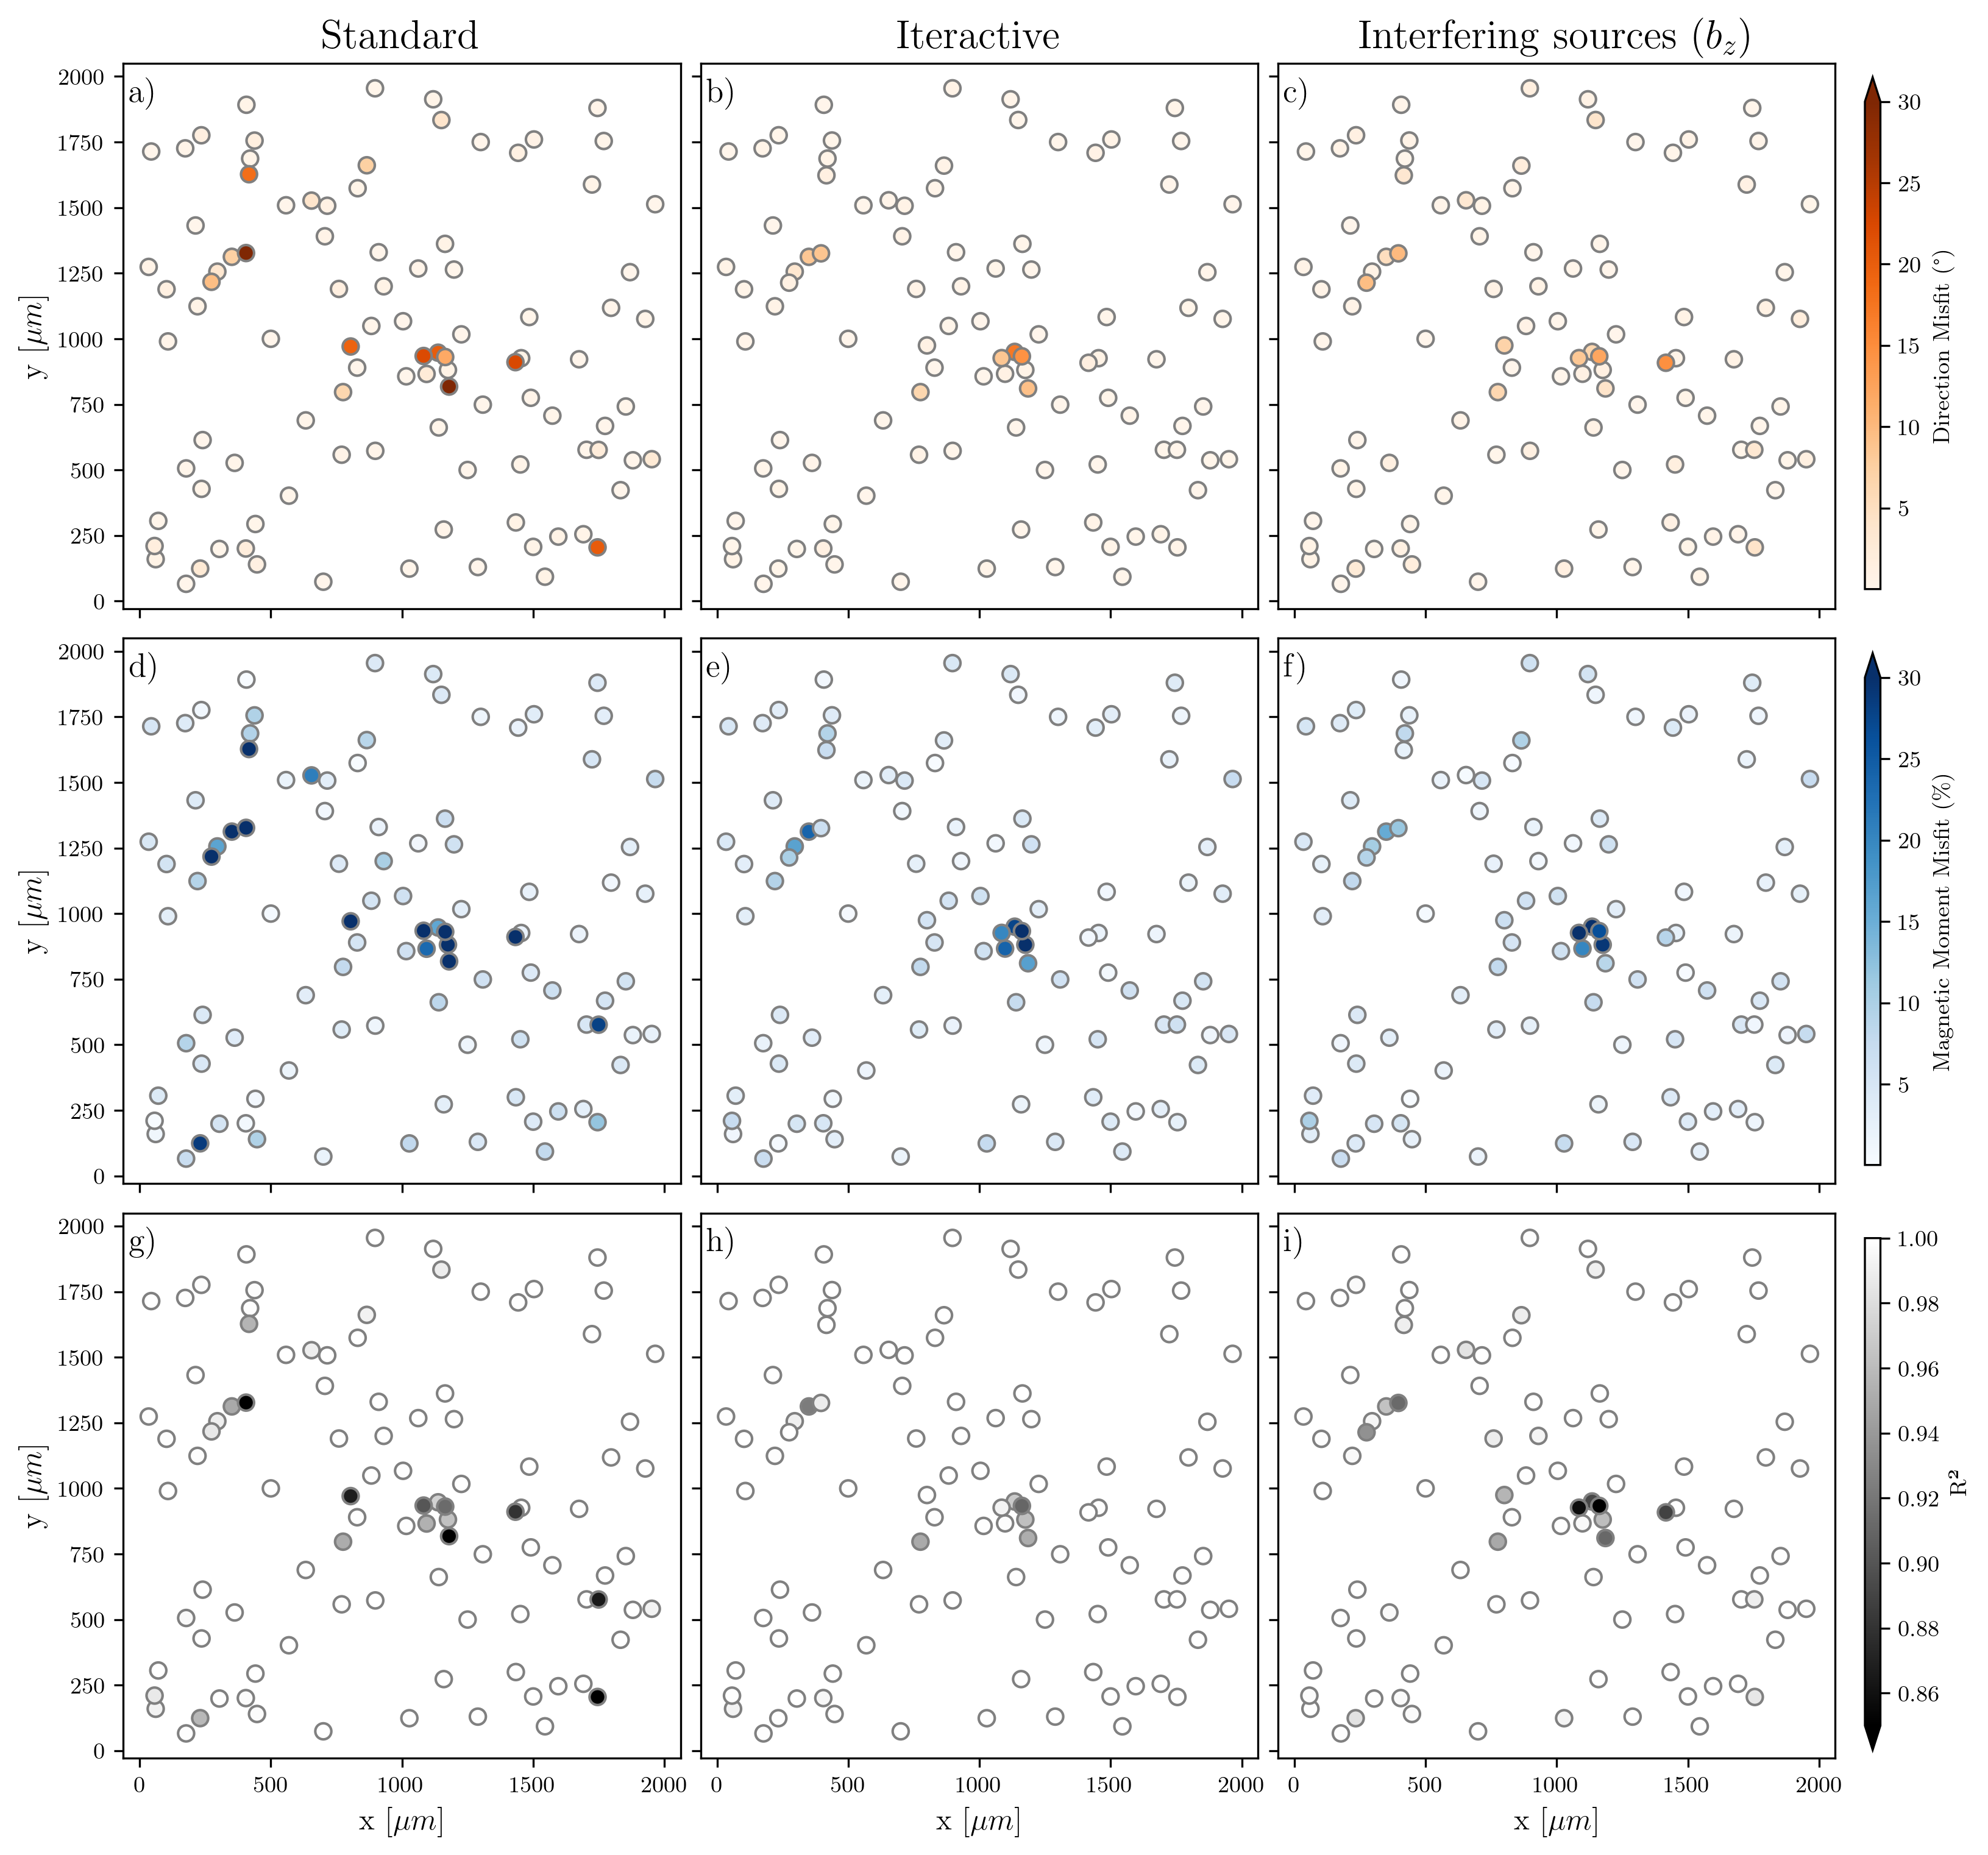
\includegraphics[width=1\linewidth]{figures/inversion-comparion-1.png}
  \caption{
    % Addressing computational challenges in magnetic microscopy with extensive datasets.
    % a) Complete synthetic dataset featuring all N observation points including areas lacking relevant information.
    % b) Streamlining data through pre-selected windows reduces the dataset size for inversion, ensuring efficiency without compromising final results.
      }
  \label{inversion1}
\end{figure}


\subsection{Shifted magnetic field acquisition}

To assess the proposed interference source techniques' ability to deal with shifted data, often observed in real magnetic microscopic data, a polynomial shift was added to the $b_z$ data vector in the previous scenario setup. 
LINKING SENTENCE
In macro-scale potential field geophysical surveys, when there is a discernible indication of a low-frequency component compromising the dataset, it becomes necessary to employ techniques that can separate the contributions of the long-wavelength (``regional'') and the short-wavelength (``residual'') components, the latter is usually associated with the targeted bodies in the studies. This requirement holds for magnetic microscopic scale acquisitions, necessitating the application of a regional-residual separation technique. To accomplish this, a first-degree polynomial fit was applied to the shifted $b_z$ magnetic field data (Figure~\ref{euler2}a) to predict the low-frequency component. This procedure was carried out using the Verde Python package \citep{verde2018}. Subsequently, the low-frequency anomaly was subtracted from the shifted $b_z$ magnetic field data, as shown in Figure~\ref{euler2}b. The Euler deconvolution algorithms for the standard (Figure~\ref{euler2}c) and iterative (Figure~\ref{euler2}d) approaches were then applied and compared. It is noted a substantial improvement in the magnetic source position estimation by the iterative method. The results are very similar to what happened to the scenario in the Subsections~\ref{non-shifted}, this is most likely caused by the robustness of the derivatives, used in the Euler equation, for long-wavelength signals.

\begin{figure}[tb!]
  \centering
  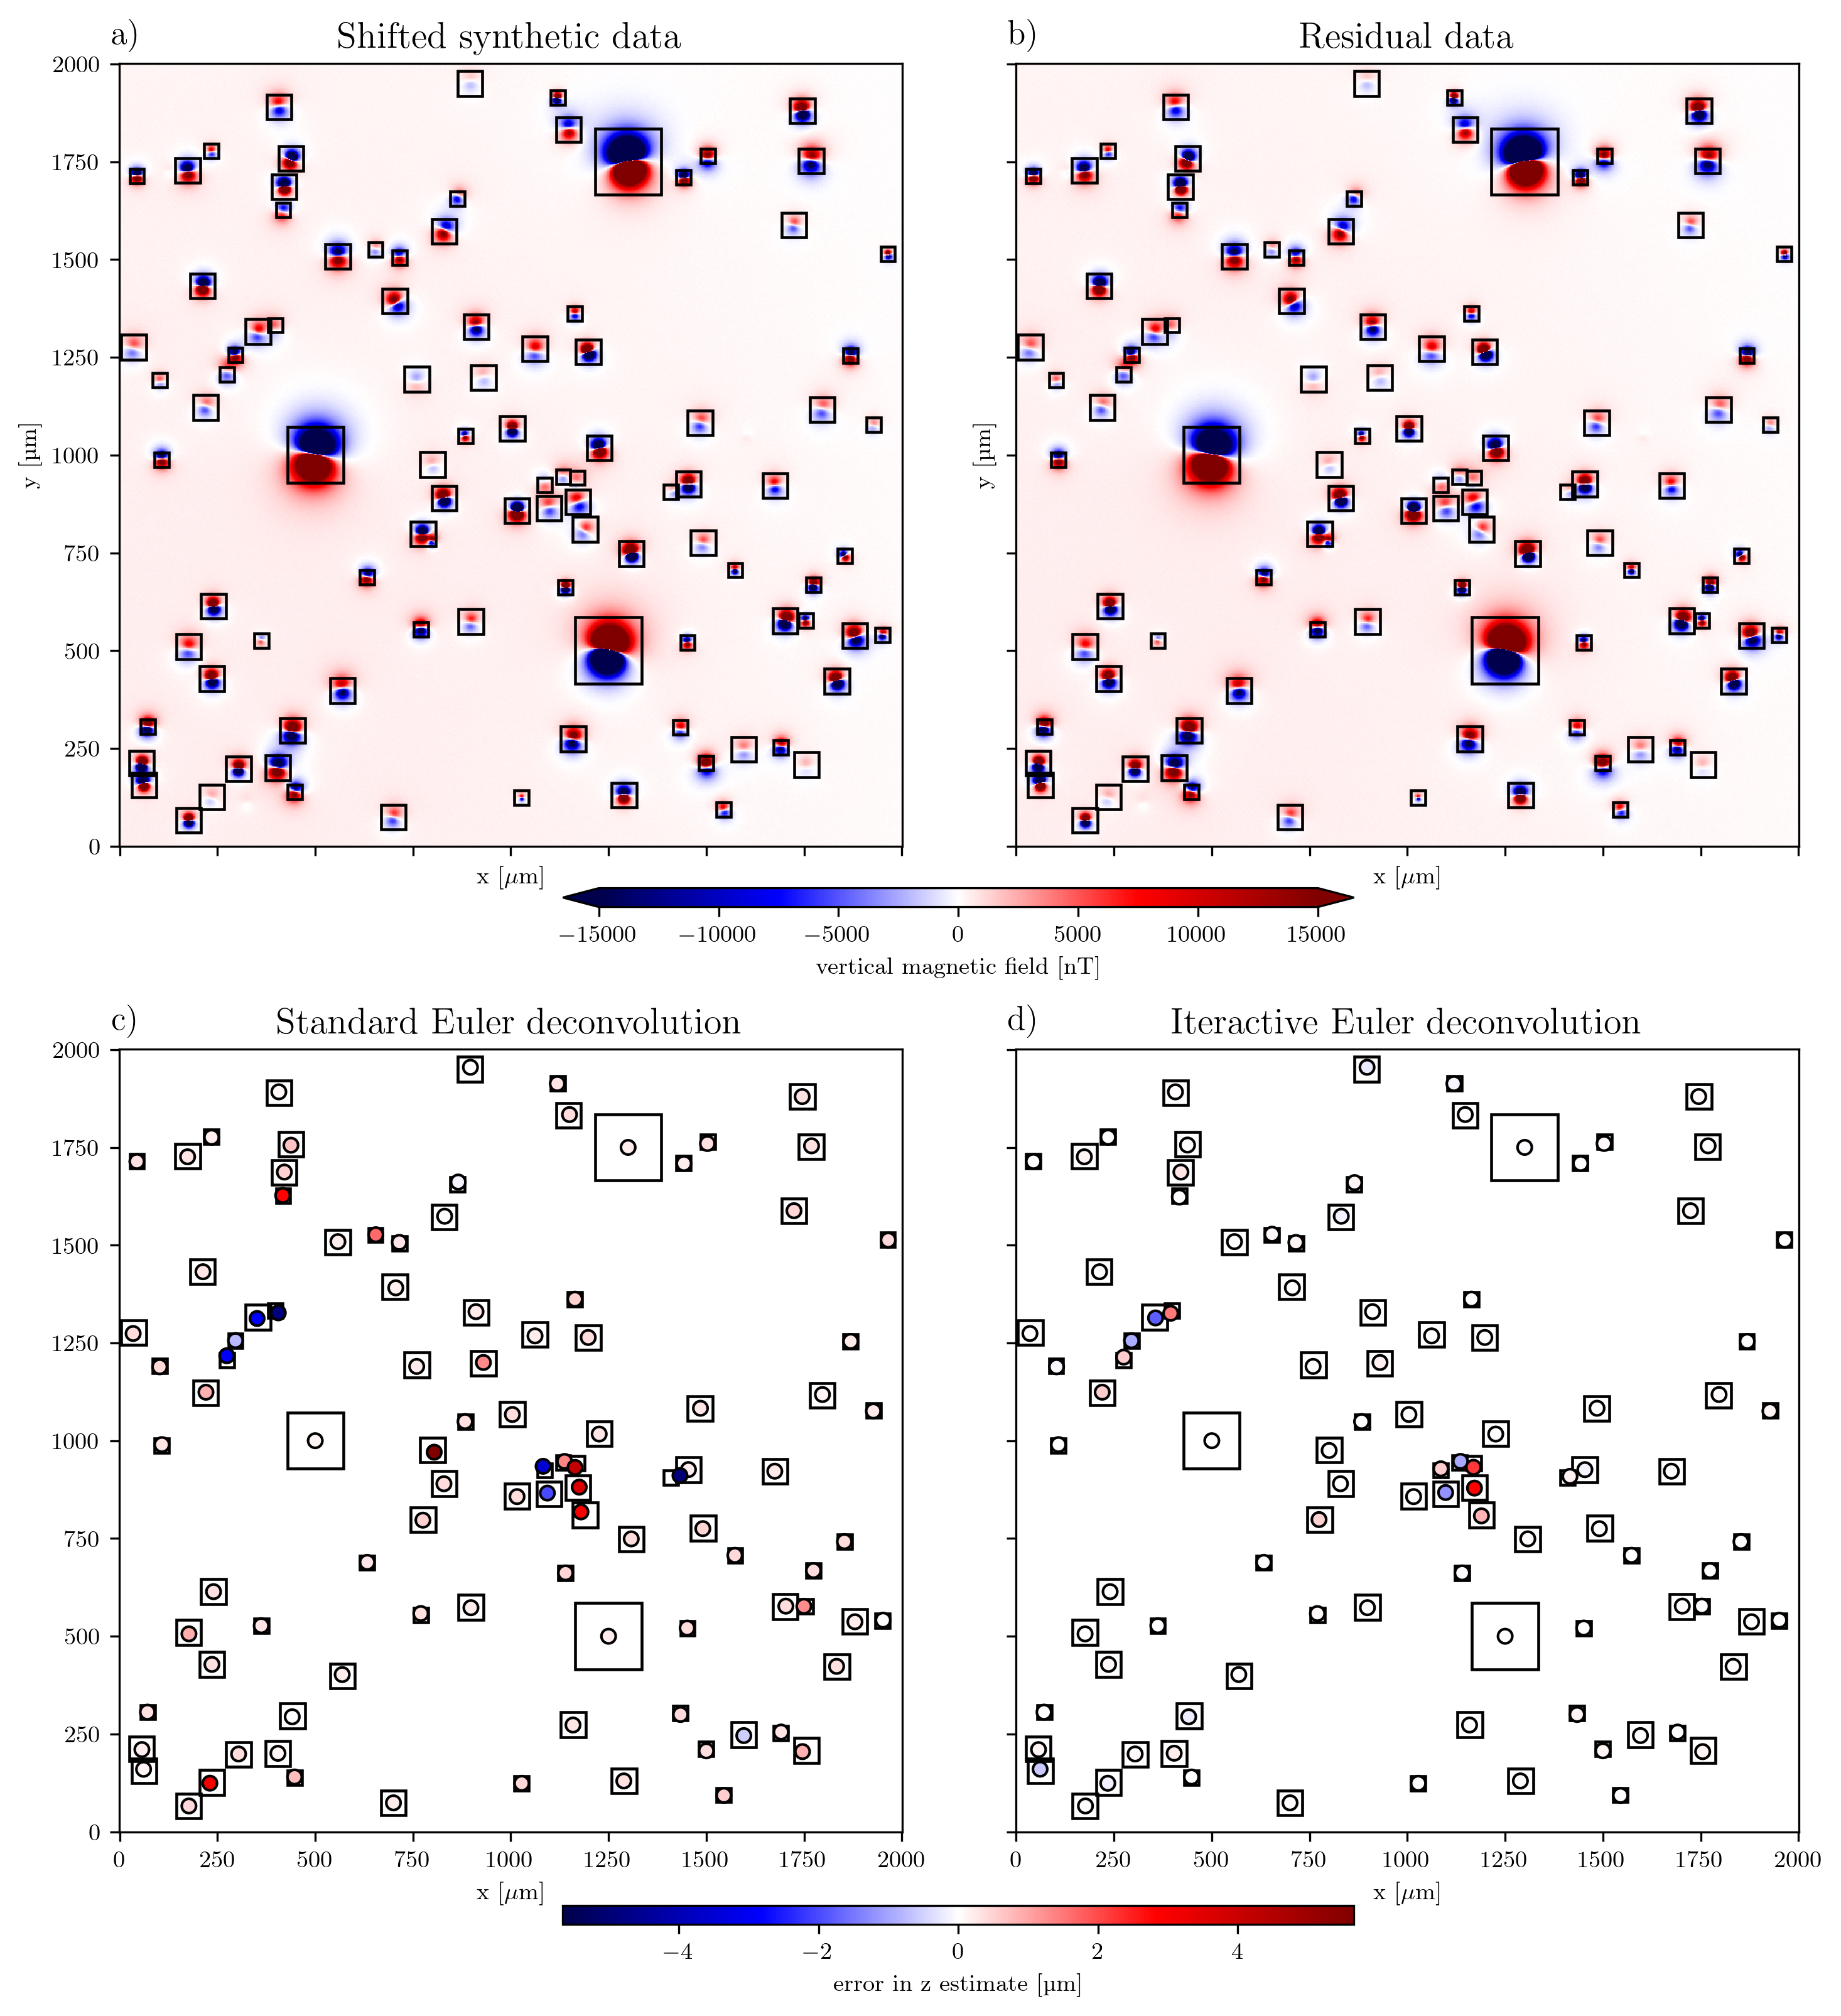
\includegraphics[width=1\linewidth]{figures/euler-comparion-2.png}
  \caption{
    % Addressing computational challenges in magnetic microscopy with extensive datasets.
    % a) Complete synthetic dataset featuring all N observation points including areas lacking relevant information.
    % b) Streamlining data through pre-selected windows reduces the dataset size for inversion, ensuring efficiency without compromising final results.
      }
  \label{euler2}
\end{figure}

Figure~\ref{inversion2} succinctly presents a comprehensive comparison encompassing angular misfit, magnetic moment misfit, and the r-squared score. The comparison is made across standard inversion results (Figures~\ref{inversion2}a-c), iterative inversion results for interfering sources (Figures~\ref{inversion2}d-f), interference with $b_z$ (Figures~\ref{inversion2}g-i), and interfering sources using the vertical derivative (Figures~\ref{inversion2}j-l). Differently from what was observed in the previous subsection, only the iterative and interfering sources using vertical derivative techniques consistently outperformed the standard method. Both techniques remained unaffected by the shift in the magnetic field, as well as the standard one. However, this pattern somehow changed for the interference source using $b_z$. Even though this technique yielded errors seemingly lower than the ones from the standard methodology, concerning the magnetic direction and moment misfit, it also demonstrated high variability in the results (not shown here) according to the shift in the magnetic field and the regional-residual separation technique used. For example, comparing the magnetic grains in the upper left region of Figure~\ref{euler2}b with Figure~\ref{inversion2}g it is clear that the sudden increase in the direction misfit is closely related to the region where the polynomial fit failed to remove the long-wavelength interference. This is also reflected in the r-squared score (Figure~\ref{inversion2}i), which makes this specific approach highly dependent on an ideal separation method. Based on this scenario, it seems that the iterative and interfering sources using the vertical derivative approaches might be more reliable for magnetic microscopy studies.

\begin{figure}[tb!]
  \centering
  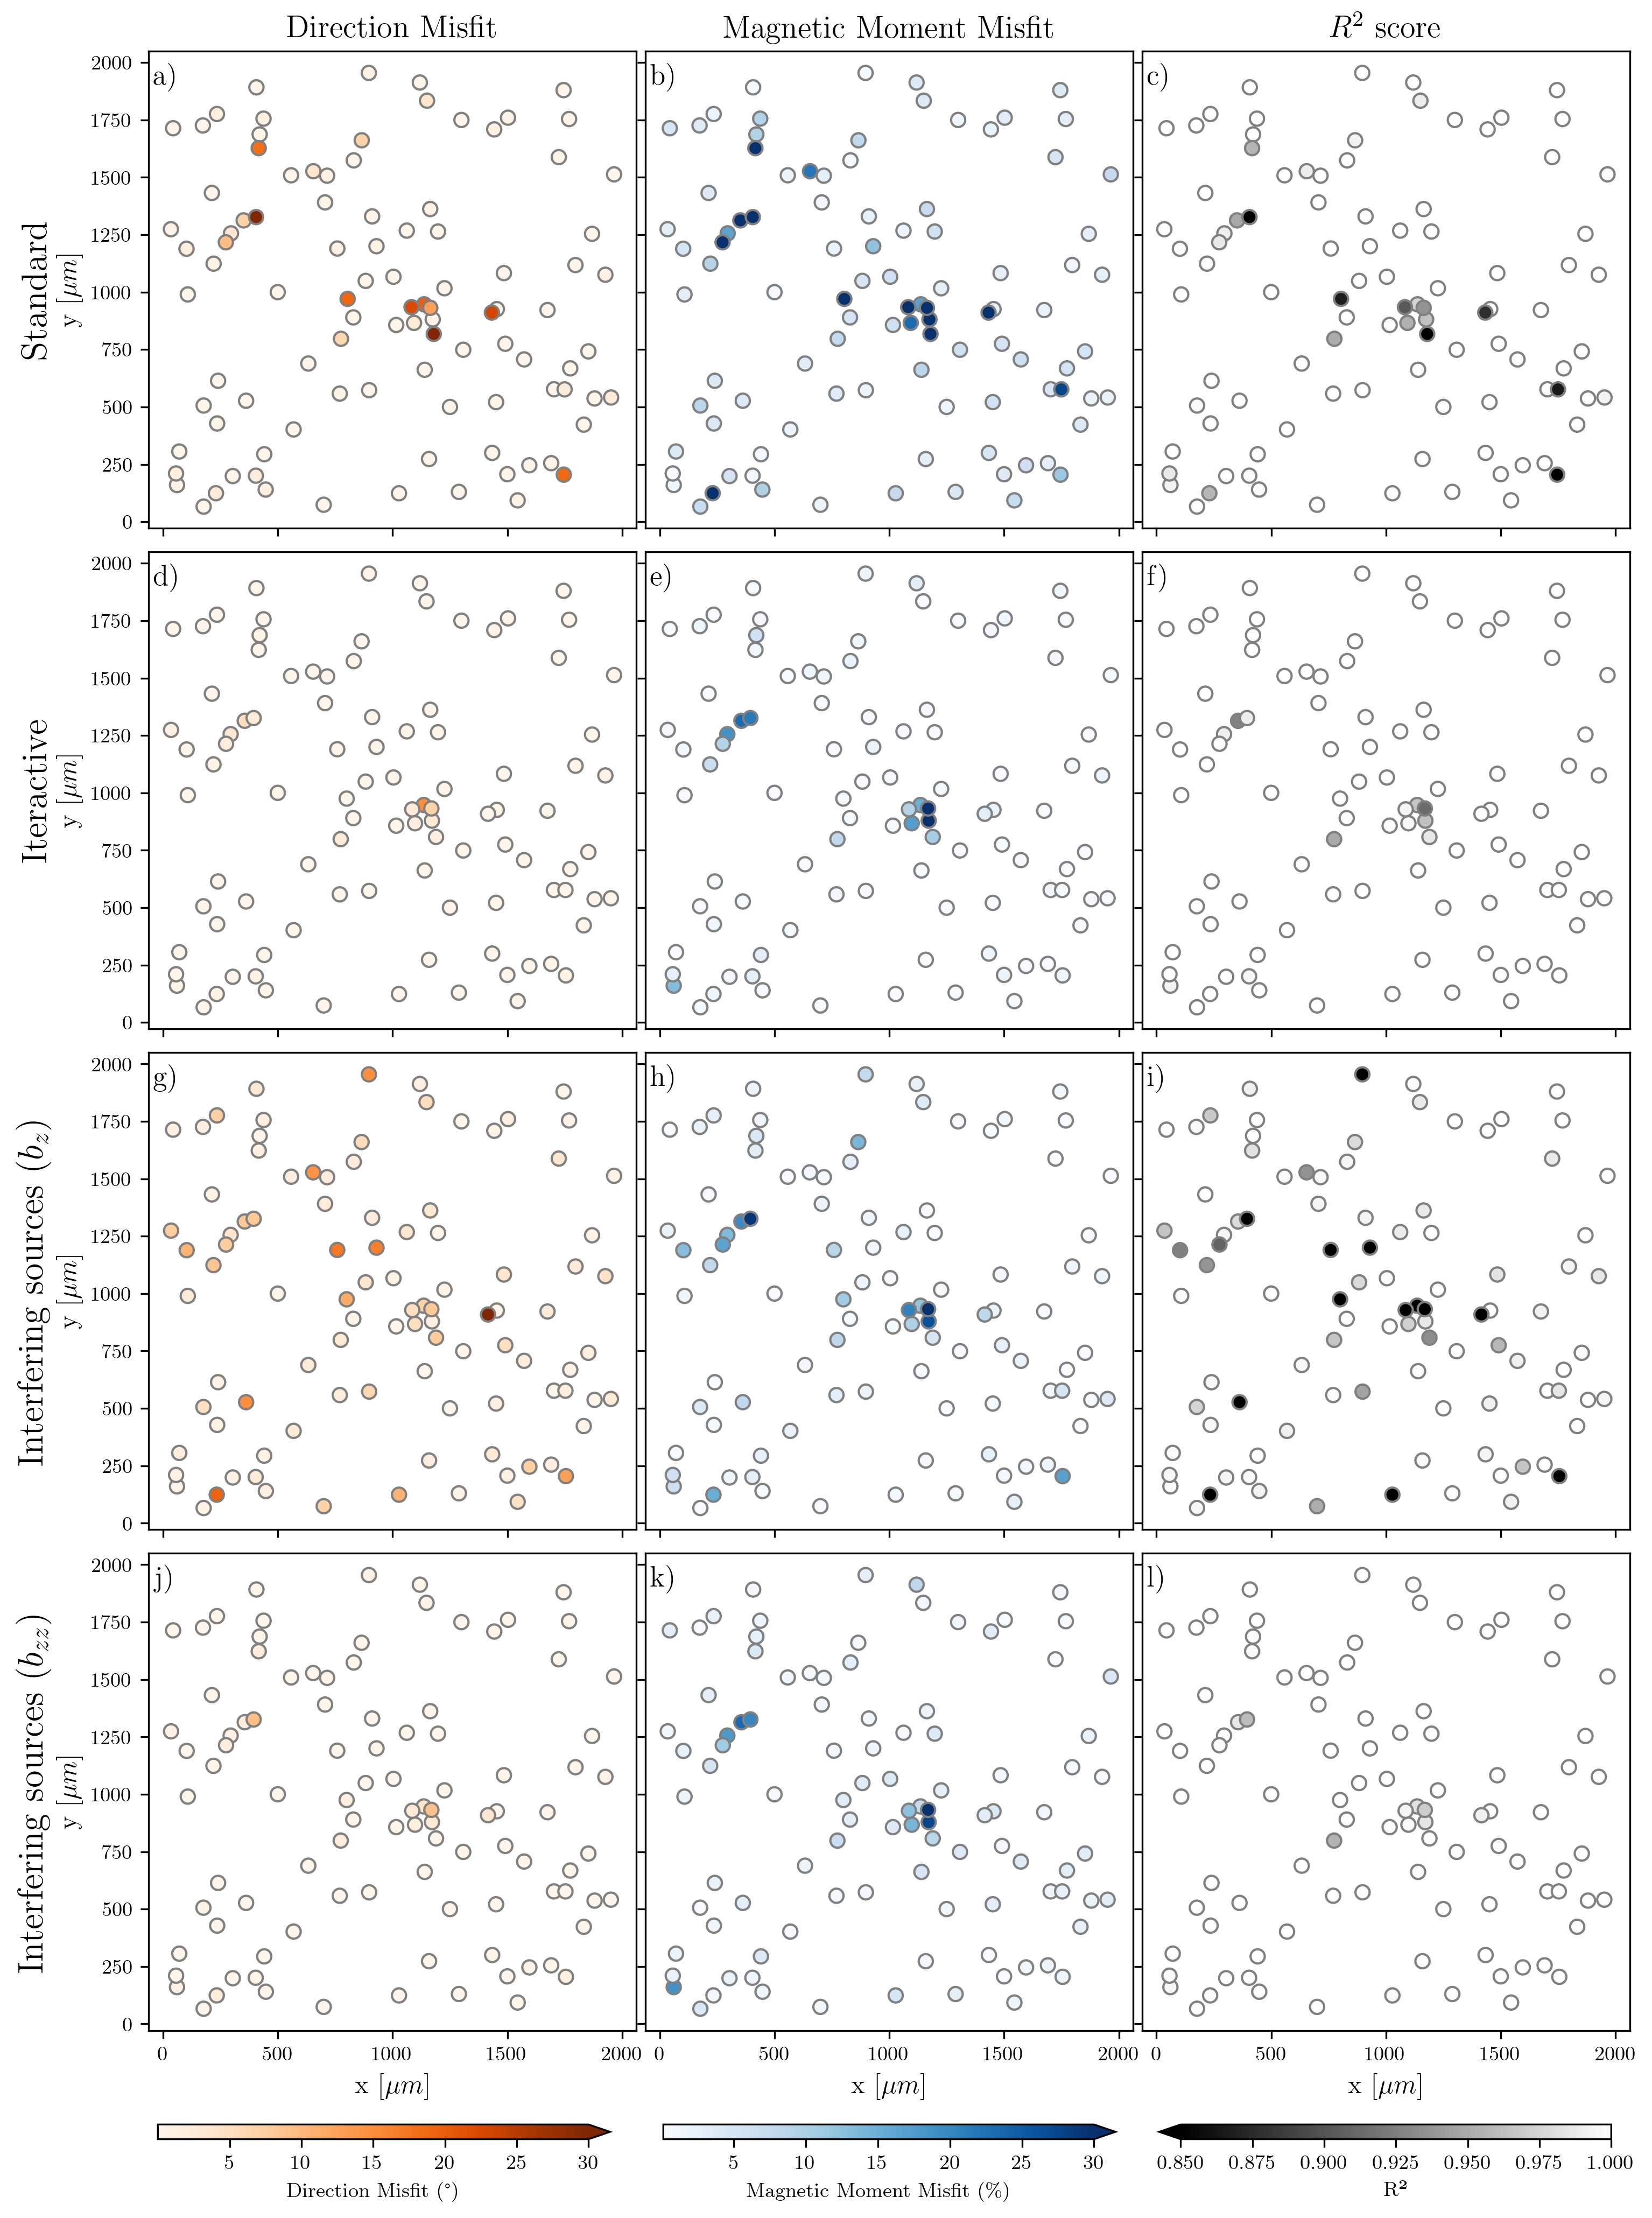
\includegraphics[width=1\linewidth]{figures/inversion-comparion-2.png}
  \caption{
    % Addressing computational challenges in magnetic microscopy with extensive datasets.
    % a) Complete synthetic dataset featuring all N observation points including areas lacking relevant information.
    % b) Streamlining data through pre-selected windows reduces the dataset size for inversion, ensuring efficiency without compromising final results.
      }
  \label{inversion2}
\end{figure}


\bibliographystyle{apalike-doi}
\bibliography{references}

\end{document}
